\chapter{Introduction}
\label{intro}

\textit{This chapter presents the overall theme of this body of work. Firstly, some context is given about the overall theme of this body of work and the motivation behind it. Then, the objectives for dissertation are presented to the reader. Finally, at the end of the chapter, some information regarding the content of each chapter is presented.}


\section{Water Supply Systems}
\label{intro:s:water-supply-systems}

The water supply systems that are prevalent in our society play a very important role in our daily lives, distributing water throughout the country from water reservoirs or water treatment plants up until it reaches our houses and industries. These \gls{wss} can be quite complex and difficult to manage without proper processes that ensure the operation of such networks is made without problems, in an environmental and economically sustainable way. For this reason, the use of specialized software to aid operators or even automatically control the operation of these \gls{wss} is of uttermost importance nowadays. Water, be it in quantity and quality, has been a staple of all major human civilizations throughout History, from ancient roman aqueducts to the current era. 

Moving large quantities of water through enormous \gls{wss} requires the use of vast quantities of mechanical work, which in turn requires lots of energy, namely, electric energy. With the ever-growing political, economic and environmental pressure to improve and optimize how we use energy, and with the current geopolitical issues, access to energy is getting more expensive and regulated. This means that the need for the optimization of pumping operations to reduce costs and, potentially lower energy use as well, is growing within \gls{wu}.

\section{Existing Decision Support System}
\label{intro:s:existing-decision-support-system}

In order for the \gls{wu}'s to optimally operate their water pumps, a \gls{dss} is used by the \gls{wu}'s pump operators and/or by automatic \gls{scada} systems. This \gls{dss} is a web platform designed to suggest \textit{which} pumps to operate, \textit{when} to operate, for \textit{how} long to operate and in some cases what \textit{speed} their \gls{vsd}'s should operate at like shown in \Cref{fig:sanepar-example-01}
\begin{figure}[!htbp]
    \centering
    \fbox{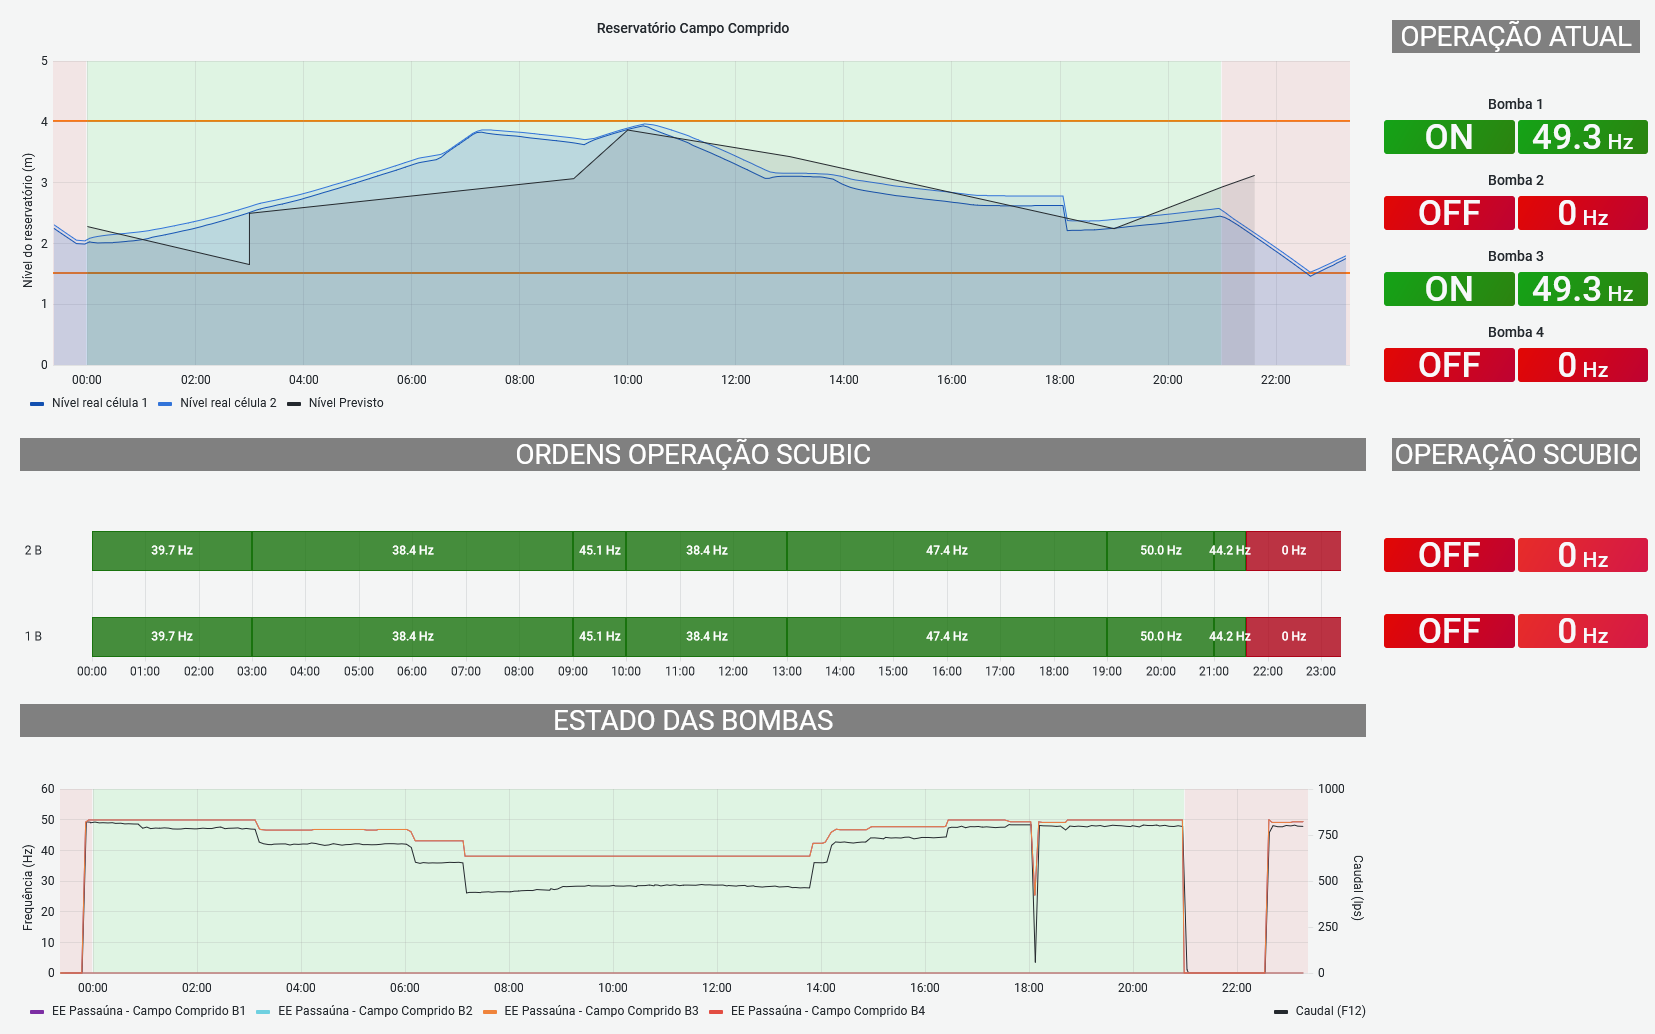
\includegraphics[width=0.95\textwidth]{img/screenshots/sanepar-example-01.png}}
    \caption[DSS example.]{Example of a \gls{dss} interface from one of SCUBIC's Clients}
    \label{fig:sanepar-example-01}
\end{figure}
    
The existing software’s architecture can be summarized as a “Monolithic Modular” software architecture \parencite{newman2019monolith}. This architecture is composed of a set of \gls{vps}, one for each Client, where a set of Docker containers contain (containers contain?) all the services needed for running the software for that Client. These services are also configured and developed separately, each in a different code repository and as such there is an unsurmountable amount of code drift between the same services of the different clients. This is, quite apparently, not scalable nor even remotely manageable for any software development team. Further ahead, on \Cref{methodology:ss:current-architecture}, a complete analysis of this architecture will be provided and explained in detail.

\section{Objectives}
\label{intro:s:objectives}

The main goal of this work is to make the migration from the old software architecture of the \gls{dss} to a better, improved software, considering the requirements from the stakeholders.
This new architecture hopes to improve the performance, reliability, resilience, security and scalability of the old \gls{dss} Architecture. A new, better architecture software brings improvements not just for the software itself but also for the development team, allowing them to improve and maintain the software easier and faster than ever before. By reducing the amount of work and time the software development team spends on each maintenance action or new functionality, it’s also hoped to save monetary resources to the software company as well. Infrastructure costs are also an important aspect of this new architecture, where the adoption of more modular and independent services might mean a more optimal use of compute resources, resulting in lowering such costs.


\section{Structure of the Document}
\label{intro:s:structure-of-the-document}

This document is composed by a total of X chapters.

In \Cref{intro}, the reader is presented with a summary of the work to be done as well as the context behind such decision.

In \Cref{state-of-the-art}, a bibliographical analysis regarding the state of software architecture and cloud-based software solutions is presented. It’s divided in two sections, starting with some insight into how a Software Architecture is planned, executed and then analyzed. Some text regarding the general technologies used throughout the work is also analyzed here.

\Cref{methodology} is divided into multiple sections. Firstly, a more detailed explanation of the old architecture and its inherent flaws is presented, flaws which end up showcasing the need for a new and improved software architecture. The second section is related to the first step when engaging a new engineering project: Requirements. In this section, the goals for the new architecture are laid out along the multiple constraints that are in place throughout the whole execution of the work. Here, the methodology to be adopted for this work is presented as well. In a third section, the plans for implementing the new architecture are laid out, chronologically. There wasn’t a single plan because the requirements and constraints kept changing during the planning and implementation part of the work. Lastly, the final section is related to the actual implementation of the proposed software architecture. The procedures taken, the challenges and decisions made throughout the implementation are shown and contextualized in this section. In here, the finalized architecture is shown with the help of diagrams. (Where can/should I introduce the methodology for measuring the performance indexes and other benchmarks that analyze the new architecture?)

\Cref{results-and-discussion} is where we can see whether the new architecture complies with the restraints imposed by the stakeholders, achieves the required and desired results and how it compares with the old architecture. In a first part, we analyze the functional requirements, followed by the non-functional requirements and overall feedback from the development team that accompanied this software architecture migration. Finally, a cost analysis is made for both the recurring monetary infrastructure costs and overall impact on team productivity.

\Cref{conclusion} discusses the previous results and presents some conclusions from what has been demonstrated on previous chapters.

Furthermore, attached to this document, is an appendix that contains some extra results generated from the monitoring interface used internally to evaluate the new architecture.

% \subsection{Options}
% \label{c1:ss:options}

% The following options are supported:

% \begin{itemize}

% \item
% \texttt{oldLogo}: to use the old logo of University of Aveiro.

% \item
% \texttt{newLogo}: to use the new logo of University of Aveiro (default behavior).

% \item
% \texttt{MAP}: for MAP joint doctoral programmes. The logos from the three universities (Aveiro, Minho, Porto) are used.

% \item
% \texttt{draft}: it prints ``DOCUMENTO PROVISÓRIO'' in the first two front pages.

% \item
% \texttt{draftPT}: same as \texttt{draft}.

% \item
% \texttt{draftEN}: same as \texttt{draft}, but instead it prints ``DRAFT DOCUMENT''.

% \item
% As of May 29, 2021, the department name shall not appear in the cover and the first page (top header).
% A new option, \texttt{NODEPT} (no department), was created to suppress the department name (now this is the default behavior).\\
% However, formerly the department name would appear in the cover and first page, therefore the old options were kept for the sake of preservation.
% Any department name can be shown by using one of the following options: \texttt{DAO}, \texttt{DBIO}, \texttt{DCM}, \texttt{DCSPT}, \texttt{DECA}, \texttt{DECIVIL}, \texttt{DEGEIT}, \texttt{DEM}, \texttt{DEMAC}, \texttt{DEP}, \texttt{DETI}, \texttt{DFIS}, \texttt{DGEO}, \texttt{DLC}, \texttt{DMAT}, \texttt{DQ}.

% \item
% The color of the top bar, in the cover page, is defined by specifying one of the following scientific areas: \texttt{accounting}, \texttt{arts}, \texttt{economy}, \texttt{education}, \texttt{engineering}, \texttt{health}, \texttt{humanities}, \texttt{sciences}.

% \end{itemize}
